% Options for packages loaded elsewhere
\PassOptionsToPackage{unicode}{hyperref}
\PassOptionsToPackage{hyphens}{url}
%
\documentclass[
]{book}
\usepackage{amsmath,amssymb}
\usepackage{lmodern}
\usepackage{iftex}
\ifPDFTeX
  \usepackage[T1]{fontenc}
  \usepackage[utf8]{inputenc}
  \usepackage{textcomp} % provide euro and other symbols
\else % if luatex or xetex
  \usepackage{unicode-math}
  \defaultfontfeatures{Scale=MatchLowercase}
  \defaultfontfeatures[\rmfamily]{Ligatures=TeX,Scale=1}
\fi
% Use upquote if available, for straight quotes in verbatim environments
\IfFileExists{upquote.sty}{\usepackage{upquote}}{}
\IfFileExists{microtype.sty}{% use microtype if available
  \usepackage[]{microtype}
  \UseMicrotypeSet[protrusion]{basicmath} % disable protrusion for tt fonts
}{}
\makeatletter
\@ifundefined{KOMAClassName}{% if non-KOMA class
  \IfFileExists{parskip.sty}{%
    \usepackage{parskip}
  }{% else
    \setlength{\parindent}{0pt}
    \setlength{\parskip}{6pt plus 2pt minus 1pt}}
}{% if KOMA class
  \KOMAoptions{parskip=half}}
\makeatother
\usepackage{xcolor}
\usepackage{longtable,booktabs,array}
\usepackage{calc} % for calculating minipage widths
% Correct order of tables after \paragraph or \subparagraph
\usepackage{etoolbox}
\makeatletter
\patchcmd\longtable{\par}{\if@noskipsec\mbox{}\fi\par}{}{}
\makeatother
% Allow footnotes in longtable head/foot
\IfFileExists{footnotehyper.sty}{\usepackage{footnotehyper}}{\usepackage{footnote}}
\makesavenoteenv{longtable}
\usepackage{graphicx}
\makeatletter
\def\maxwidth{\ifdim\Gin@nat@width>\linewidth\linewidth\else\Gin@nat@width\fi}
\def\maxheight{\ifdim\Gin@nat@height>\textheight\textheight\else\Gin@nat@height\fi}
\makeatother
% Scale images if necessary, so that they will not overflow the page
% margins by default, and it is still possible to overwrite the defaults
% using explicit options in \includegraphics[width, height, ...]{}
\setkeys{Gin}{width=\maxwidth,height=\maxheight,keepaspectratio}
% Set default figure placement to htbp
\makeatletter
\def\fps@figure{htbp}
\makeatother
\setlength{\emergencystretch}{3em} % prevent overfull lines
\providecommand{\tightlist}{%
  \setlength{\itemsep}{0pt}\setlength{\parskip}{0pt}}
\setcounter{secnumdepth}{5}
\newlength{\cslhangindent}
\setlength{\cslhangindent}{1.5em}
\newlength{\csllabelwidth}
\setlength{\csllabelwidth}{3em}
\newlength{\cslentryspacingunit} % times entry-spacing
\setlength{\cslentryspacingunit}{\parskip}
\newenvironment{CSLReferences}[2] % #1 hanging-ident, #2 entry spacing
 {% don't indent paragraphs
  \setlength{\parindent}{0pt}
  % turn on hanging indent if param 1 is 1
  \ifodd #1
  \let\oldpar\par
  \def\par{\hangindent=\cslhangindent\oldpar}
  \fi
  % set entry spacing
  \setlength{\parskip}{#2\cslentryspacingunit}
 }%
 {}
\usepackage{calc}
\newcommand{\CSLBlock}[1]{#1\hfill\break}
\newcommand{\CSLLeftMargin}[1]{\parbox[t]{\csllabelwidth}{#1}}
\newcommand{\CSLRightInline}[1]{\parbox[t]{\linewidth - \csllabelwidth}{#1}\break}
\newcommand{\CSLIndent}[1]{\hspace{\cslhangindent}#1}
\usepackage{booktabs}
\usepackage{amsthm}
\makeatletter
\def\thm@space@setup{%
  \thm@preskip=8pt plus 2pt minus 4pt
  \thm@postskip=\thm@preskip
}
\makeatother
\usepackage{booktabs}
\usepackage{longtable}
\usepackage{array}
\usepackage{multirow}
\usepackage{wrapfig}
\usepackage{float}
\usepackage{colortbl}
\usepackage{pdflscape}
\usepackage{tabu}
\usepackage{threeparttable}
\usepackage{threeparttablex}
\usepackage[normalem]{ulem}
\usepackage{makecell}
\usepackage{xcolor}
\ifLuaTeX
  \usepackage{selnolig}  % disable illegal ligatures
\fi
\usepackage[]{natbib}
\bibliographystyle{apalike}
\IfFileExists{bookmark.sty}{\usepackage{bookmark}}{\usepackage{hyperref}}
\IfFileExists{xurl.sty}{\usepackage{xurl}}{} % add URL line breaks if available
\urlstyle{same} % disable monospaced font for URLs
\hypersetup{
  pdftitle={BID: Pobreza Energética},
  hidelinks,
  pdfcreator={LaTeX via pandoc}}

\title{BID: Pobreza Energética}
\author{true}
\date{2022-08-09}

\begin{document}
\maketitle

{
\setcounter{tocdepth}{1}
\tableofcontents
}
\hypertarget{introducciuxf3n}{%
\chapter{Introducción}\label{introducciuxf3n}}

Apoyo para una Transición Energética Justa, Limpia y Sostenible en Chile:

\textbf{Estudio para la medición de indicadores de pobreza energética}

\hypertarget{objetivos}{%
\chapter{Objetivos}\label{objetivos}}

\hypertarget{objetivos-generales}{%
\section{Objetivos Generales}\label{objetivos-generales}}

Medir Indicadores de Probreza Energética en el sector residencial, con la escala más detallada posible en base a la información ya disponible en otros estudios y bases de datos, con la que actualmente cuente el Misterio, o que pueda gestionar de manera efectiva para su utilización posterior.

\hypertarget{objetivos-especuxedficos}{%
\section{Objetivos Específicos}\label{objetivos-especuxedficos}}

\begin{itemize}
\tightlist
\item
  Desarrollar y definir metodologías para la contrucción de indicadores.
\end{itemize}

\hypertarget{m_teorico}{%
\chapter{Marco Teórico}\label{m_teorico}}

\hypertarget{definiciuxf3n-de-conceptos}{%
\section{Definición de Conceptos}\label{definiciuxf3n-de-conceptos}}

\hypertarget{quuxe9-es-pobreza-energuxe9tica}{%
\subsection{¿Qué es pobreza Energética?}\label{quuxe9-es-pobreza-energuxe9tica}}

Nos referimos a Pobreza Energética cuando un hogar no tiene acceso equitativo a servicios energéticos de alta calidad (es decir, que sean adecuados, confiables, no contaminantes y seguros) para cubrir sus necesidades fundamentales y básicas que permitan sostener el desarrollo humano y económico de sus integrantes.

Un hogar se encuentra en situación de pobreza energética cuando no tiene acceso equitativo a servicios energéticos de alta calidad para cubrir sus necesidades fundamentales y básicas, que permitan sostener el desarrollo humano y económico de sus miembros. Las necesidades fundamentales son aquellas que implican impactos directos en la salud humana; mientras que las necesidades básicas corresponden a aquellos requerimientos energéticos cuya pertinencia depende de las particularidades culturales y territoriales.

\begin{figure}

{\centering 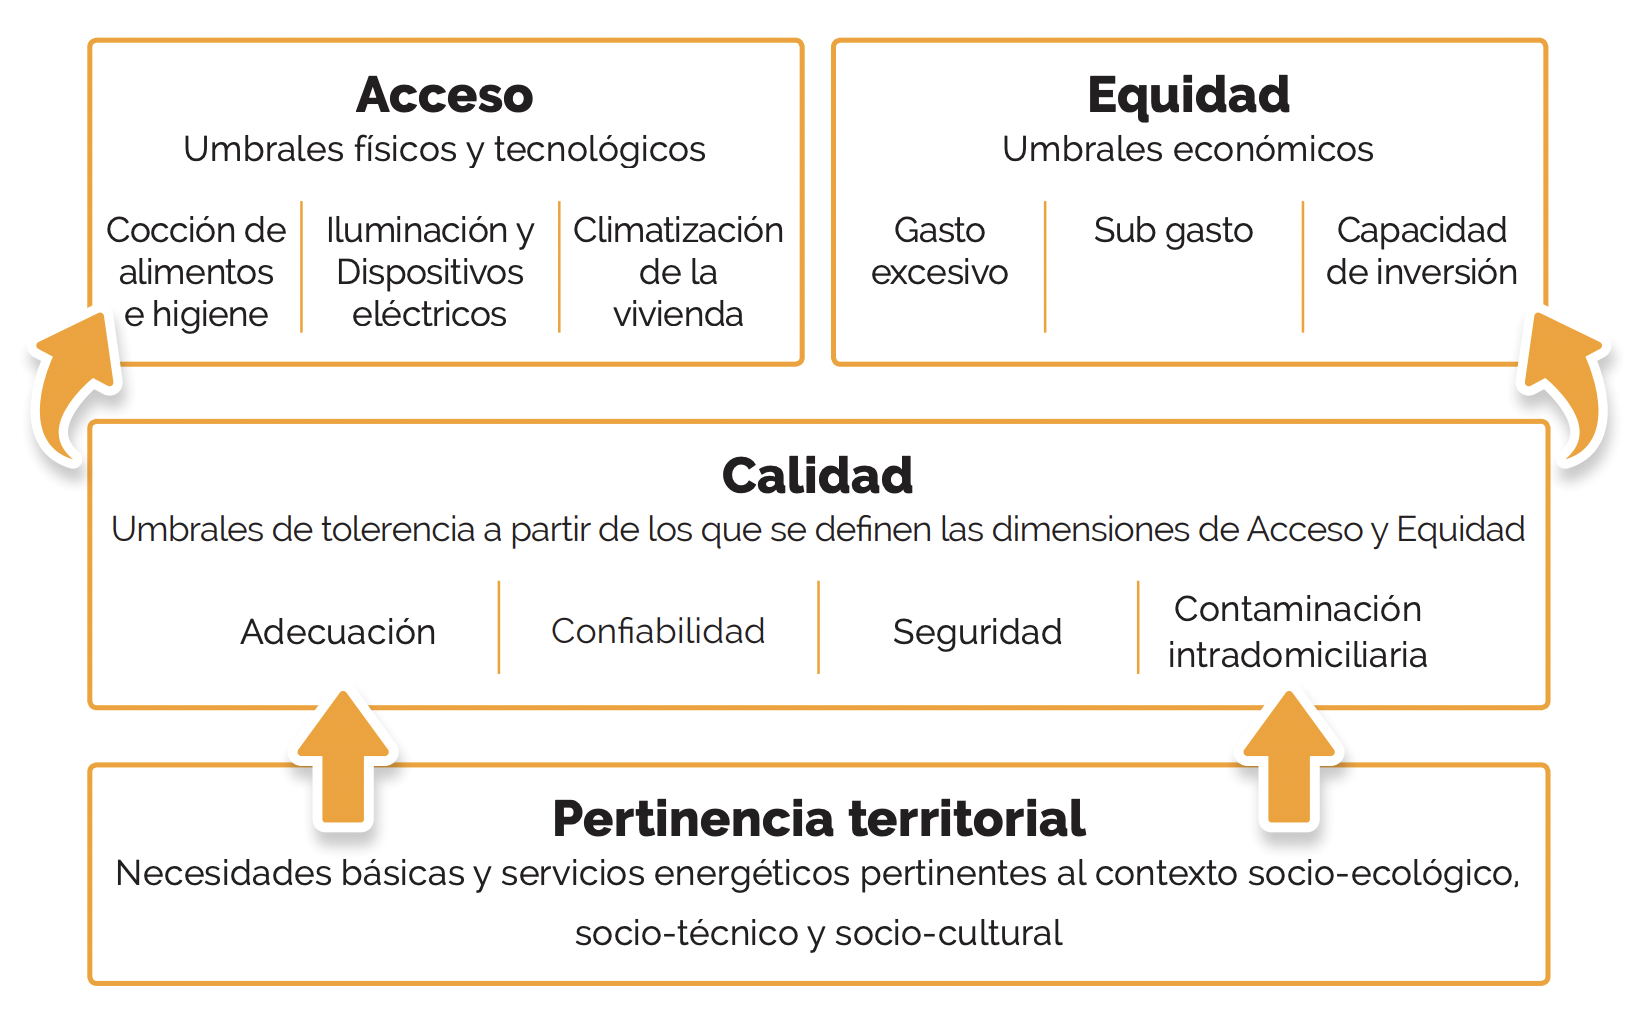
\includegraphics[width=1\linewidth]{images/esquema_PE} 

}

\caption{Esquema conceptual Pobreza Energética}\label{fig:unnamed-chunk-2}
\end{figure}

La pobreza energética se expresa en relación a dos grupos de necesidades: `\emph{fundamentales}' y `\emph{básicas}'. Las necesidades \textbf{fundamentales} son aquellas que implican impactos directos en la salud humana. Su satisfacción se considera crítica, independiente del contexto territorial. La cocción y conservación de alimentos, las temperaturas mínima y máxima saludables, el acceso al agua y la disponibilidad de suministro eléctrico continuo para personas electrodependientes en salud, se encuentran en este primer grupo. Por otra parte, las necesidades \textbf{básicas} corresponden a aquellos requerimientos cuya pertinencia depende de las características socioecológicas (biofísicas, geográficas y climáticas), sociotécnicas (tecnológicas e infraestructurales) y socioculturales (normas, mercados, costumbres y expectativas relacionadas con calidad de vida y desarrollo humano), propias de un determinado territorio. El confort térmico, el agua caliente sanitaria, la iluminación, los electrodomésticos y dispositivos tecnológicos para la educación son ejemplos de este segundo grupo.

Mientras las necesidades fundamentales se consideran de forma universal, las necesidades básicas requieren de una definición y ponderación en función de su pertinencia para una población en particular, situada en un territorio, en un contexto temporal definido y bajo condiciones socioculturales específicas.

\begin{figure}

{\centering 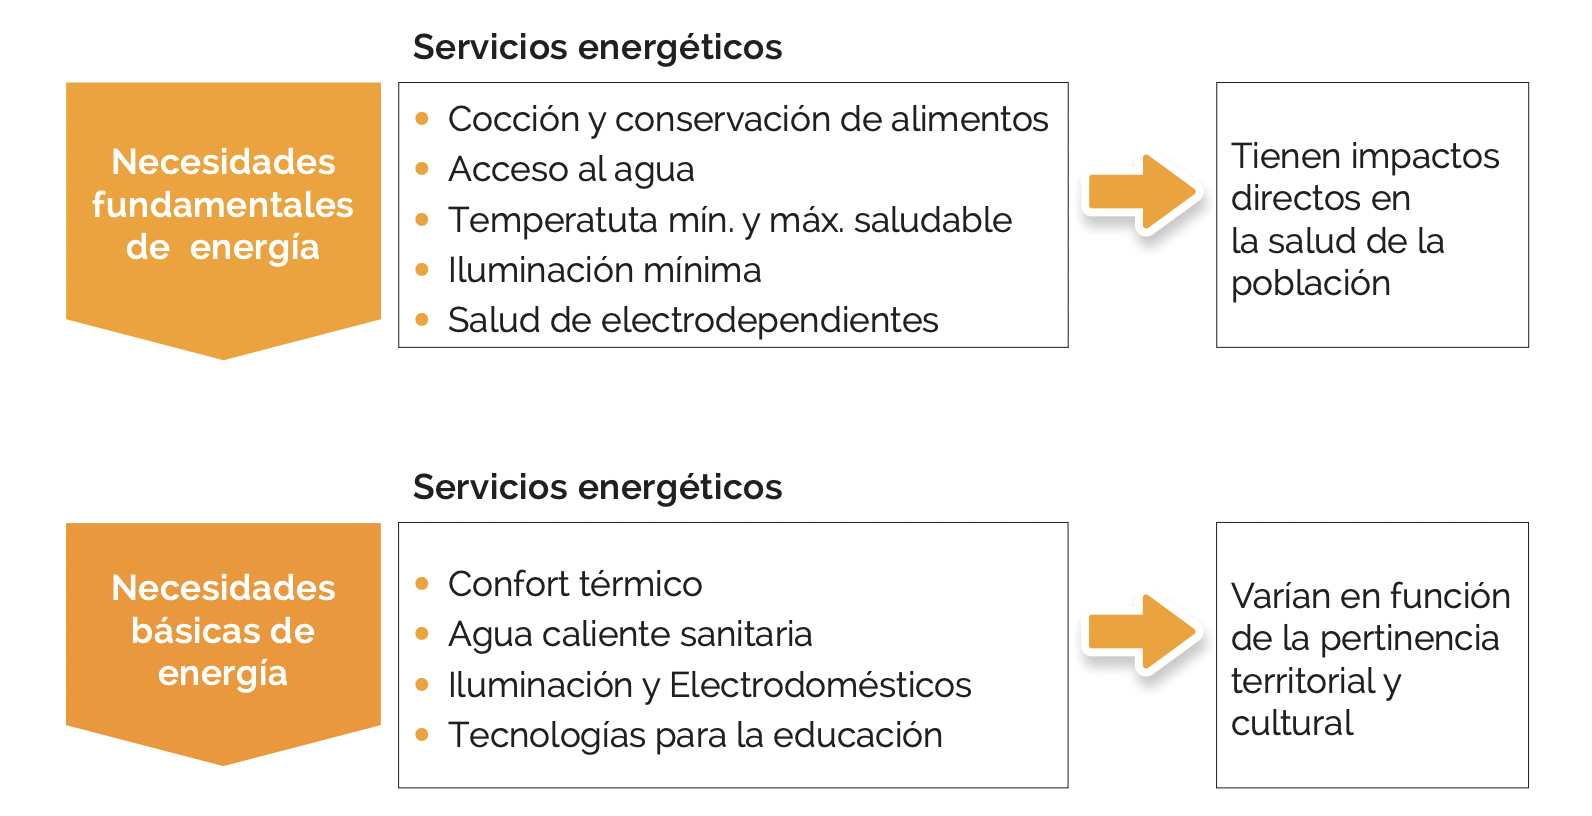
\includegraphics[width=1\linewidth]{images/necedidades_energia} 

}

\caption{Necesidades fundamentales y básica de energía}\label{fig:unnamed-chunk-3}
\end{figure}

\hypertarget{seguridad-energuxe9tica}{%
\subsection{Seguridad Energética}\label{seguridad-energuxe9tica}}

Capacidad de un territorio para garantizar acceso equitativo en cantidad y calidad a servicios energéticos resilientes y sostenibles, que permita el desarrollo económico y humano del territorio y sus habitantes. \citep{urquiza_water_2020}

\begin{figure}

{\centering 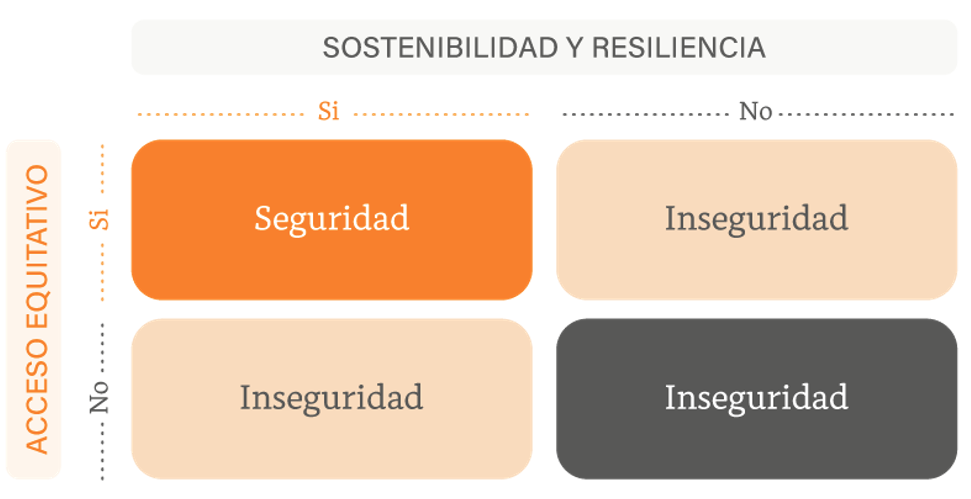
\includegraphics[width=1\linewidth]{images/seguridad_ene} 

}

\caption{Seguridad Energética}\label{fig:unnamed-chunk-4}
\end{figure}

\hypertarget{propuesta-de-indicadores}{%
\section{Propuesta de Indicadores}\label{propuesta-de-indicadores}}

\hypertarget{acceso-equitativo}{%
\subsection{Acceso Equitativo}\label{acceso-equitativo}}

\begin{figure}

{\centering 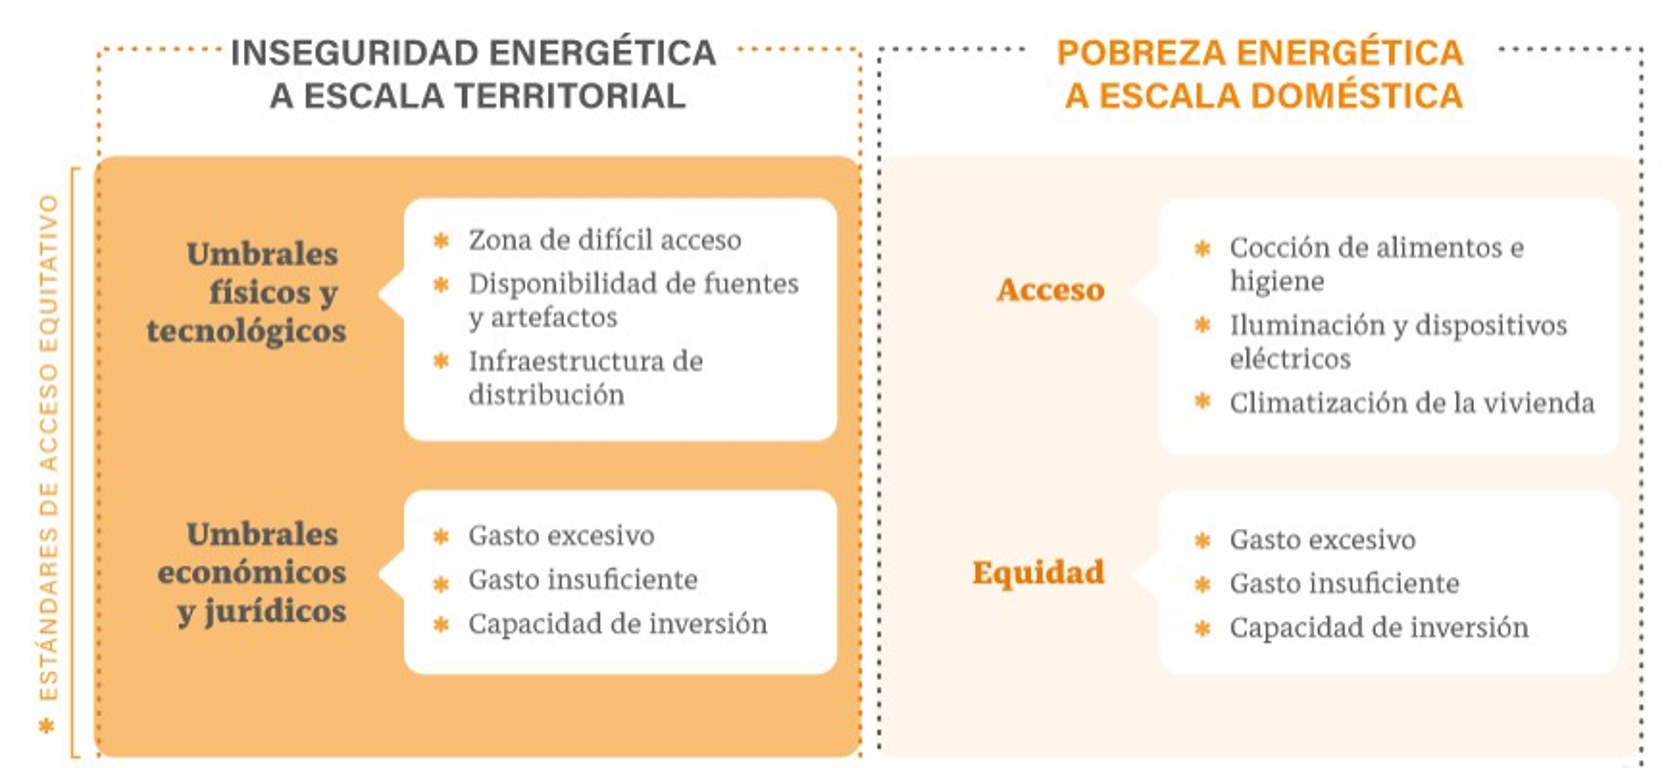
\includegraphics[width=1\linewidth]{images/a_equitativo} 

}

\caption{Estándares de acceso equitativo}\label{fig:unnamed-chunk-5}
\end{figure}

\hypertarget{calidad-y-cantidad}{%
\subsection{Calidad y Cantidad}\label{calidad-y-cantidad}}

\begin{figure}

{\centering 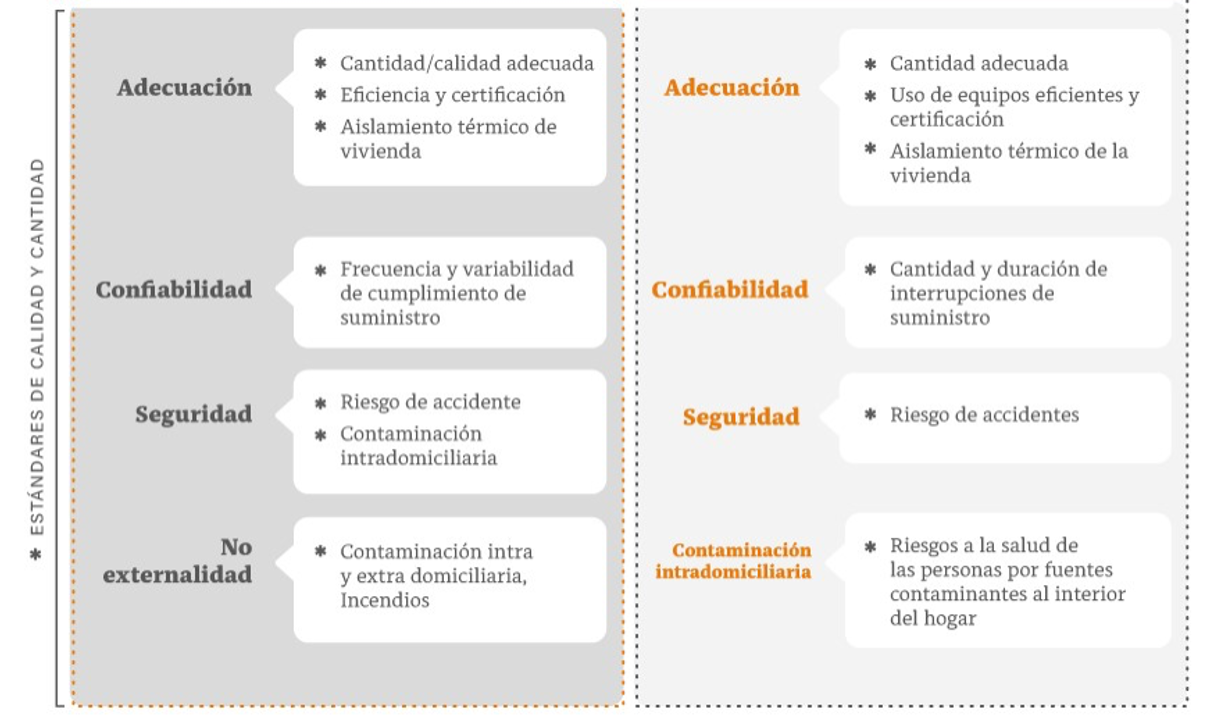
\includegraphics[width=1\linewidth]{images/calidad_cant} 

}

\caption{Estándares Calidad y Cantidad}\label{fig:unnamed-chunk-6}
\end{figure}

\hypertarget{indicadores-pe2050-y-consultoruxeda-bid}{%
\subsection{Indicadores PE2050 y consultoría BID}\label{indicadores-pe2050-y-consultoruxeda-bid}}

\textbf{Indicadores Consultoría BID}

\begin{itemize}
\tightlist
\item
  Consumo de energía bajo condición de confort térmico vs consumo energía real (con resolución a nivel de manzana y temporalidad a ser definida)
\item
  Gasto mensual de energía bajo condición de confort térmico vs gasto en situación real (con resolución a nivel de manzana y temporalidad a ser definida)
\item
  Otro criterio prioritario es segmentar en base a distintas variables socio económicas (al menos nivel socio económico, pertinencia indígena y género)
\end{itemize}

\textbf{Indicadores Política Energética 2050}

\begin{itemize}
\tightlist
\item
  Porcentaje de hogares con acceso a electricidad de forma permanente respecto al total de hogares existentes.
\item
  Porcentaje de hogares que acceden a calefacción, agua caliente sanitaria y cocción de alimentos a partir de fuentes de energía limpias de bajas emisiones.
\item
  Gasto energético en el hogar (contrastado con definición establecida de gasto asequible). Se pueden considerar 3 indicadores: gasto excesivo (gasto que ubica al hogar bajo la línea de pobreza al considerar el ingreso y los otros gastos), sub-gasto (gasto menor al de hogares similares, implicando que no se alcanza el confort térmico), y porcentaje de las principales categorías de artefactos y equipos que se venden en el mercado que corresponden a equipos energéticamente eficientes.
\item
  Porcentaje de viviendas que tienen un acondicionamiento térmico equivalente a la reglamentación térmica 2021 y 2031, del total del parque construido.
\end{itemize}

\hypertarget{indicadores-internacionales}{%
\section{Indicadores Internacionales}\label{indicadores-internacionales}}

\begin{figure}

{\centering 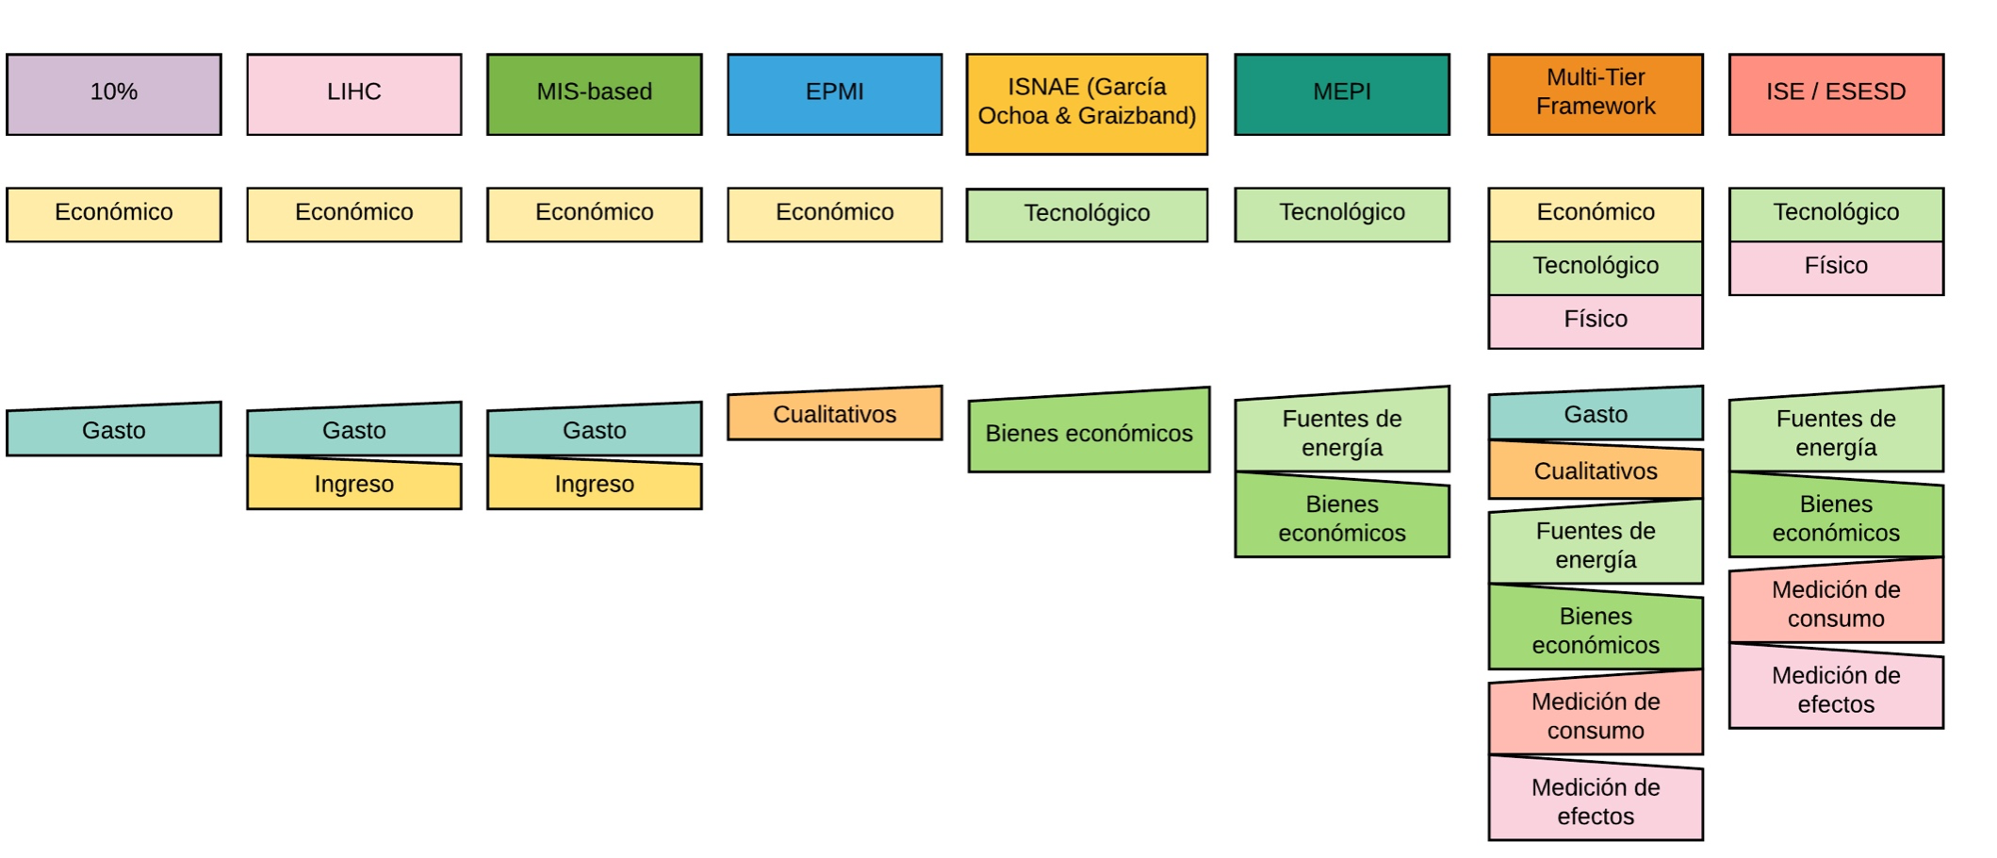
\includegraphics[width=1\linewidth]{images/ind_internacionales} 

}

\caption{Indicadores Internacionales}\label{fig:unnamed-chunk-7}
\end{figure}

\hypertarget{propuesta-indicadores}{%
\section{Propuesta Indicadores}\label{propuesta-indicadores}}

\begin{figure}

{\centering 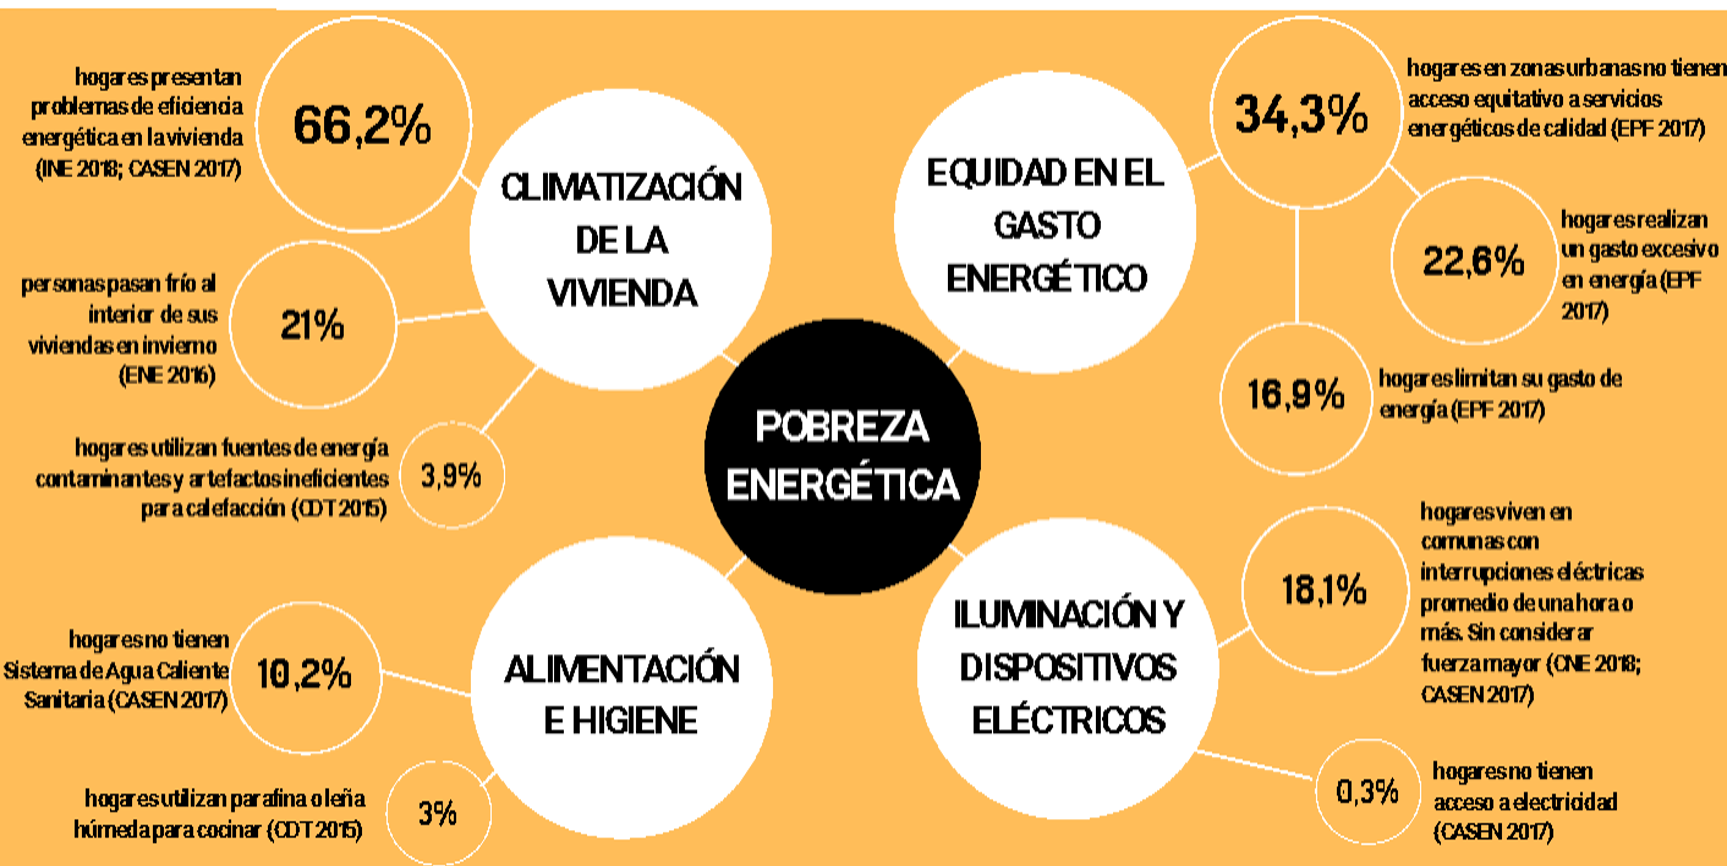
\includegraphics[width=1\linewidth]{images/esquema_indicadores} 

}

\caption{Esquema de propuesta des Indicadores}\label{fig:unnamed-chunk-8}
\end{figure}

\hypertarget{data_explorer}{%
\chapter{Exploración de Datos}\label{data_explorer}}

Las bases de datos recibidas de Probreza Energética (27-07-2022), corresponden a 3 carpetas, las cuales en el presente capítulo se procederá un análisis descriptivo general.

\begin{figure}
\centering
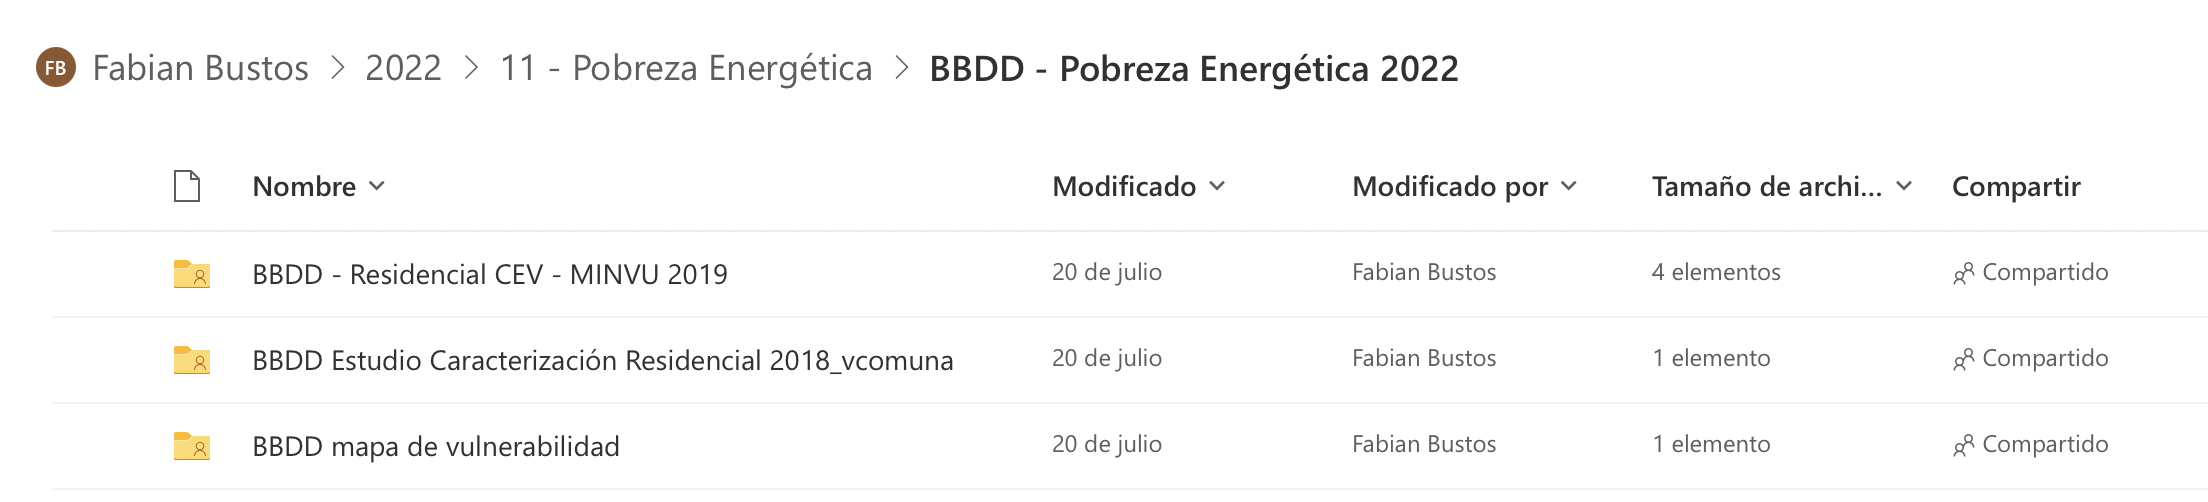
\includegraphics{images/bbdd_folders.png}
\caption{Estructura de carpeta de Bases de Datos}
\end{figure}

\hypertarget{bbdd-mapa-vulneravilidad}{%
\section{BBDD mapa vulneravilidad}\label{bbdd-mapa-vulneravilidad}}

\hypertarget{descripciuxf3n-de-variables}{%
\subsection{Descripción de Variables}\label{descripciuxf3n-de-variables}}

\textbf{Nombre Archivo}: ``\emph{Detalle de campos.xlsx}''

\begingroup\fontsize{11}{13}\selectfont

\begin{tabu} to \linewidth {>{\centering}X>{\centering}X>{\centering}X}
\hline
Nombre campo & Descripción & Fuente\\
\hline
REGION & Código región & INE, Censo 2017\\
\hline
PROVINCIA & Código provincia & INE, Censo 2017\\
\hline
COMUNA & Código comuna & INE, Censo 2017\\
\hline
NOM\_REGION & Nombre región & INE, Censo 2017\\
\hline
NOM\_PROVIN & Nombre provincia & INE, Censo 2017\\
\hline
NOM\_COMUNA & Nombre comuna & INE, Censo 2017\\
\hline
DESTINO\_VI & Uso o destino de la vivienda 
2: vivienda colectiva
3: vivienda de temporada
4: vivienda desocupada
5: vivienda ocupada con moradores ausentes
6: vivienda ocupada con moradores presentes & INE, Pre censo 2016\\
\hline
NOM\_DIRECC & Nombre de calle o camino de referencia & INE, Pre censo 2016\\
\hline
N\_LETRA & Numeración & INE, Pre censo 2016\\
\hline
LOCALIDAD & Nombre de localidad, área rural & INE, Censo 2017\\
\hline
ENTIDAD & Nombre de entidad, área rural & INE, Censo 2017\\
\hline
CATEGORIA & Nombres de categorías de asentamiento humano en área rural & INE, Censo 2017\\
\hline
EMPRESA\_ID & Identificador empresa distribuidora & SEC, 2018\\
\hline
EMPRESA\_1 & Nombre empresa distribuidora & SEC, 2018\\
\hline
SSAA & 1: vivienda se ubica en sistema aislado
0: vivienda no se ubica en sistema aislado & Catastro SSAA, 2018\\
\hline
NOM\_SSAA & Nombre del sistema aislado & Catastro SSAA, 2018\\
\hline
TIPO\_SUM\_S & Tipo de suministro del sistema eléctrico aislado: 
Parcial: menos de 24 horas al día
Permanente: 24 horas al día & Catastro SSAA, 2018\\
\hline
FV\_IND & 1: vivienda tiene sistema individual de autogeneración
0: vivienda no tiene sistema individual de autogeneración & Catastro sistemas individuales, 2018\\
\hline
NOM\_FV\_IND & Nombre del proyecto que dio origen al sistema individual & Catastro sistemas individuales, 2018\\
\hline
SUMINS\_FV & Tipo de suministro del sistema individual: 
Parcial: menos de 24 horas al día
Permanente: 24 horas al día & Catastro sistemas individuales, 2018\\
\hline
PROY\_ELECT & 1: vivienda está incluida en algún proyecto de electrificación
0: vivienda no está incluida en algún proyecto de electrificación & Varias fuentes\\
\hline
EST\_PROY\_E & Estado del proyecto: ejecutado, en ejecución, RS, con financiamiento, en licitación. & Varias fuentes\\
\hline
NOM\_PRO\_EL & Nombre del proyecto & Varias fuentes\\
\hline
CODIGO\_IDI & Código IDI del proyecto (código del banco integrado de proyectos) & Varias fuentes\\
\hline
X & Longitud & Obtenida en Arcgis\\
\hline
Y & Latitud & Obtenida en Arcgis\\
\hline
\end{tabu}
\endgroup{}

\hypertarget{analisis-bases-espaciales}{%
\subsection{Analisis Bases Espaciales}\label{analisis-bases-espaciales}}

Dentro de la carpeta llamada \texttt{BBDD\ mapa\ vulneravilidad} existen 4 archivos en formato shapefiles, con los siguientes nombres:

\begin{itemize}
\tightlist
\item
  viv\_proy
\item
  viv\_sin\_energia
\item
  viv\_sist\_aislado
\item
  viv\_sist\_indiv
\end{itemize}

Para visualizar los objetos esjetos espaciales se procedió a elegir una región de COQUIMBO, continiación se procede a hacer exploración de las tablas de contenidos y visualización espacial por cada uno de ellos:

\hypertarget{viv_proy}{%
\subsubsection{viv\_proy}\label{viv_proy}}

\textbf{Tabla de Variables}:

\begin{table}
\centering\begingroup\fontsize{10}{12}\selectfont

\begin{tabular}{c|c|c|c|c|c|c|c|c|c|c|c|c|c|c|c|c|c|c|c|c|c|c|c|c|c}
\hline
REGION & NOM\_REGION & PROVINCIA & NOM\_PROVIN & COMUNA & NOM\_COMUNA & DESTINO\_VI & NOM\_DIRECC & N\_LETRA & EMPRESA\_ID & EMPRESA\_1 & DISTRITO & AREA & COD\_LOCALI & LOCALIDAD & COD\_ENTIDA & ENTIDAD & COD\_CATEGO & CATEGORIA & EST\_PROY\_E & NOM\_PRO\_EL & CODIGO\_IDI & NEAR\_DIST & MANZENT\_I & X & Y\\
\hline
04 & COQUIMBO & 042 & CHOAPA & 04203 & LOS VILOS & 6 & SN & SN & 7 & CONAFE & 5 & 2 & 23 & LOS CÓNDORES & 58 & EL LLANO & 8 & PARCELA-HIJUELA & RS & ELECTRIFICACION RURAL VALLE DE QUILIMARI & 30094239 & 41.720 & 4.203052e+12 & -71.304 & -32.092\\
\hline
04 & COQUIMBO & 042 & CHOAPA & 04203 & LOS VILOS & 6 & SN & SN & 7 & CONAFE & 5 & 2 & 16 & INFIERNILLO & 46 & INFIERNILLO & 8 & PARCELA-HIJUELA & RS & ELECTRIFICACION RURAL VALLE DE QUILIMARI & 30094239 & 28.217 & 4.203052e+12 & -71.299 & -32.079\\
\hline
04 & COQUIMBO & 042 & CHOAPA & 04203 & LOS VILOS & 6 & SN & SN & 7 & CONAFE & 4 & 2 & 23 & LOS CÓNDORES & 66 & RINCONADA & 8 & PARCELA-HIJUELA & RS & ELECTRIFICACION RURAL VALLE DE QUILIMARI & 30094239 & 83.881 & 4.203042e+12 & -71.242 & -32.078\\
\hline
04 & COQUIMBO & 042 & CHOAPA & 04203 & LOS VILOS & 6 & SN & SN & 18 & CGED & 5 & 2 & 16 & INFIERNILLO & 46 & INFIERNILLO & 8 & PARCELA-HIJUELA & EN EJECUCION & ELECTRIFICACION RURAL INFIERNILLO II & 30073621 & 367.058 & 4.203052e+12 & -71.311 & -32.041\\
\hline
04 & COQUIMBO & 042 & CHOAPA & 04203 & LOS VILOS & 6 & SN & SN & 18 & CGED & 5 & 2 & 16 & INFIERNILLO & 46 & INFIERNILLO & 8 & PARCELA-HIJUELA & EN EJECUCION & ELECTRIFICACION RURAL INFIERNILLO II & 30073621 & 327.209 & 4.203052e+12 & -71.310 & -32.041\\
\hline
\end{tabular}
\endgroup{}
\end{table}

\textbf{Visualización Espacial}: Región de ``COQUIMBO''

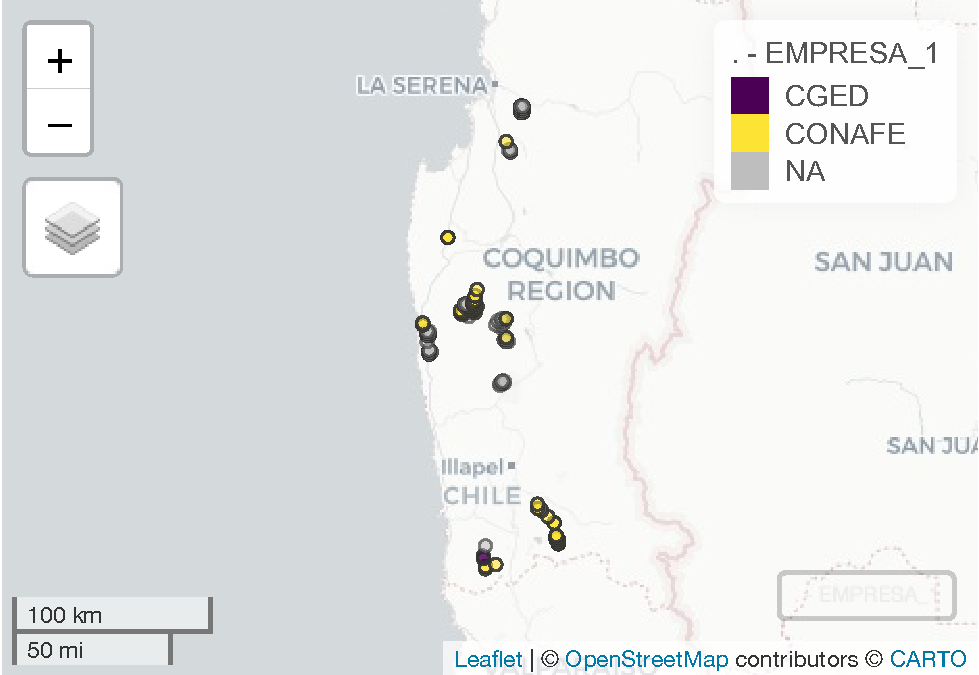
\includegraphics{bookdown_BID_PE_files/figure-latex/unnamed-chunk-14-1.pdf}

\hypertarget{viv_sin_energia}{%
\subsubsection{viv\_sin\_energia}\label{viv_sin_energia}}

\textbf{Tabla de Variables}:

\begin{table}
\centering\begingroup\fontsize{10}{12}\selectfont

\begin{tabular}{c|c|c|c|c|c|c|c|c|c|c|c|c|c|c|c|c|c|c|c|c|c|c|c}
\hline
NUMERAL & REGION & NOM\_REGION & PROVINCIA & NOM\_PROVIN & COMUNA & DISTRITO & AREA & COD\_LOCALI & LOCALIDAD & COD\_ENTIDA & ENTIDAD & COD\_CATEGO & CATEGORIA & MANZENT\_I & DESTINO\_VI & NOM\_DIRECC & N\_LETRA & EMPRESA\_ID & EMPRESA\_1 & NEAR\_DIST & Y & X & NOM\_COMUNA\\
\hline
24 & 04 & COQUIMBO & 042 & CHOAPA & 04203 & 6 & 2 & 15 & GUANGUALÍ & 42 & LO CLAUDIO & 8 & PARCELA-HIJUELA & 4.203062e+12 & 6 & SN & SN & 7 & CONAFE & 952.030 & -32.174 & -71.362 & LOS VILOS\\
\hline
78 & 04 & COQUIMBO & 042 & CHOAPA & 04203 & 7 & 2 & 32 & QUILIMARÍ & 96 & EL ARRAYÁN AFUERA & 8 & PARCELA-HIJUELA & 4.203072e+12 & 6 & SN & SN & 0 & NA & 3545.851 & -32.155 & -71.443 & LOS VILOS\\
\hline
79 & 04 & COQUIMBO & 042 & CHOAPA & 04203 & 7 & 2 & 32 & QUILIMARÍ & 96 & EL ARRAYÁN AFUERA & 8 & PARCELA-HIJUELA & 4.203072e+12 & 6 & SN & SN & 0 & NA & 3552.633 & -32.155 & -71.444 & LOS VILOS\\
\hline
82 & 04 & COQUIMBO & 042 & CHOAPA & 04203 & 6 & 2 & 901 & INDETERMINADA & 901 & INDETERMINADA & 15 & INDETERMINADA & 4.203063e+12 & 6 & SN & SN & 0 & NA & 1499.775 & -32.153 & -71.341 & LOS VILOS\\
\hline
98 & 04 & COQUIMBO & 042 & CHOAPA & 04203 & 7 & 2 & 29 & PICHIDANGUI & 901 & INDETERMINADA & 15 & INDETERMINADA & 4.203072e+12 & 6 & SN & SN & 7 & CONAFE & 1166.592 & -32.147 & -71.486 & LOS VILOS\\
\hline
\end{tabular}
\endgroup{}
\end{table}

\textbf{Visualización Espacial}: Región de ``COQUIMBO''

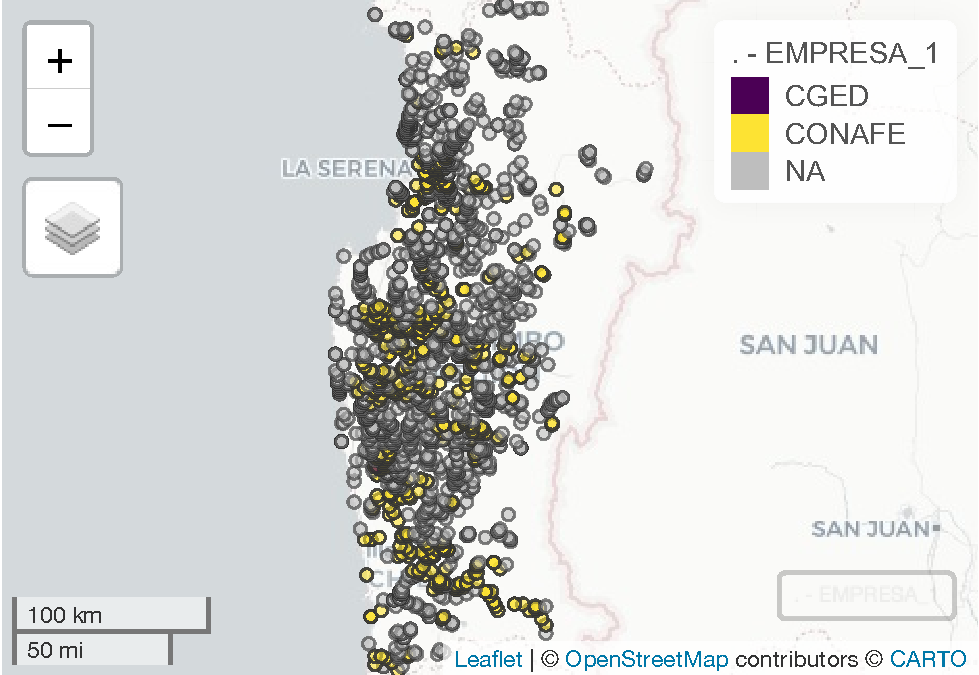
\includegraphics{bookdown_BID_PE_files/figure-latex/unnamed-chunk-18-1.pdf}

\hypertarget{viv_sist_aislado}{%
\subsubsection{viv\_sist\_aislado}\label{viv_sist_aislado}}

\textbf{Tabla de Variables}:

\begingroup\fontsize{10}{12}\selectfont

\begin{tabu} to \linewidth {>{\centering}X>{\centering}X>{\centering}X>{\centering}X>{\centering}X>{\centering}X>{\centering}X>{\centering}X>{\centering}X>{\centering}X>{\centering}X>{\centering}X>{\centering}X>{\centering}X>{\centering}X>{\centering}X>{\centering}X>{\centering}X>{\centering}X>{\centering}X>{\centering}X>{\centering}X>{\centering}X>{\centering}X>{\centering}X>{\centering}X>{\centering}X}
\hline
OBJECTID & NUMERAL & REGION & PROVINCIA & COMUNA & NOM\_REGION & NOM\_PROVIN & NOM\_COMUNA & DESTINO\_VI & NOM\_DIRECC & N\_LETRA & EMPRESA\_ID & EMPRESA\_1 & DISTRITO & AREA & COD\_LOCALI & LOCALIDAD & COD\_ENTIDA & ENTIDAD & COD\_CATEGO & CATEGORIA & MANZENT\_I & NOM\_SSAA & TIPO\_SUM\_S & NEAR\_DIST & X & Y\\
\hline
2168 & 67751 & 04 & 041 & 04101 & COQUIMBO & ELQUI & LA SERENA & 6 & AVENIDA LATORRE & SN & 0 & NA & 12 & 2 & 10 & COMUNIDAD AGRÍCOLA HISTÓRICA OLLA DE CALDERA & 78 & ALMIRANTE LATORRE & 4 & CASERÍO & 4.101122e+12 & ALMIRANTE LATORRE & PARCIAL & 21273.43 & -70.959 & -29.638\\
\hline
2169 & 67759 & 04 & 041 & 04101 & COQUIMBO & ELQUI & LA SERENA & 6 & SN & SN & 0 & NA & 12 & 2 & 10 & COMUNIDAD AGRÍCOLA HISTÓRICA OLLA DE CALDERA & 78 & ALMIRANTE LATORRE & 4 & CASERÍO & 4.101122e+12 & ALMIRANTE LATORRE & PARCIAL & 21459.73 & -70.956 & -29.637\\
\hline
2170 & 67762 & 04 & 041 & 04101 & COQUIMBO & ELQUI & LA SERENA & 6 & LOS AGUIRRE & SN & 0 & NA & 12 & 2 & 10 & COMUNIDAD AGRÍCOLA HISTÓRICA OLLA DE CALDERA & 78 & ALMIRANTE LATORRE & 4 & CASERÍO & 4.101122e+12 & ALMIRANTE LATORRE & PARCIAL & 21474.31 & -70.956 & -29.637\\
\hline
2171 & 67763 & 04 & 041 & 04101 & COQUIMBO & ELQUI & LA SERENA & 6 & SN & SN & 0 & NA & 12 & 2 & 10 & COMUNIDAD AGRÍCOLA HISTÓRICA OLLA DE CALDERA & 78 & ALMIRANTE LATORRE & 4 & CASERÍO & 4.101122e+12 & ALMIRANTE LATORRE & PARCIAL & 21520.10 & -70.955 & -29.637\\
\hline
2172 & 67771 & 04 & 041 & 04101 & COQUIMBO & ELQUI & LA SERENA & 6 & JOSE MIGUEL PIÑONES & SN & 0 & NA & 12 & 2 & 10 & COMUNIDAD AGRÍCOLA HISTÓRICA OLLA DE CALDERA & 78 & ALMIRANTE LATORRE & 4 & CASERÍO & 4.101122e+12 & ALMIRANTE LATORRE & PARCIAL & 21444.00 & -70.956 & -29.637\\
\hline
\end{tabu}
\endgroup{}

\textbf{Visualización Espacial}: Región de ``COQUIMBO''

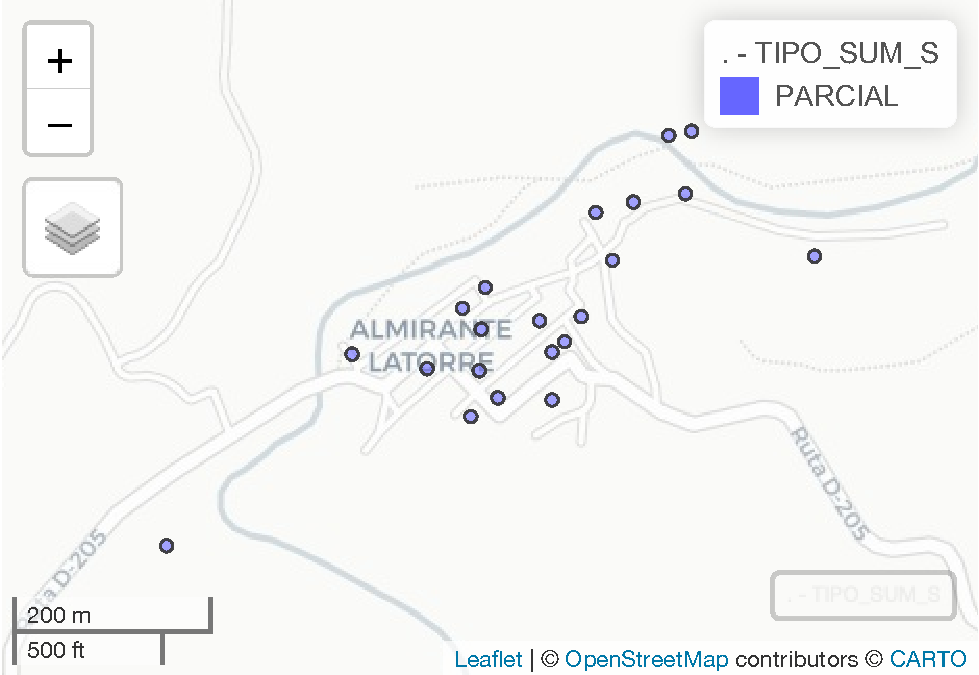
\includegraphics{bookdown_BID_PE_files/figure-latex/unnamed-chunk-22-1.pdf}

\hypertarget{viv_sist_indiv}{%
\subsubsection{viv\_sist\_indiv}\label{viv_sist_indiv}}

\textbf{Tabla de Variables}:

\begingroup\fontsize{10}{12}\selectfont

\begin{tabu} to \linewidth {>{\centering}X>{\centering}X>{\centering}X>{\centering}X>{\centering}X>{\centering}X>{\centering}X>{\centering}X>{\centering}X>{\centering}X>{\centering}X>{\centering}X>{\centering}X>{\centering}X>{\centering}X>{\centering}X>{\centering}X>{\centering}X>{\centering}X>{\centering}X>{\centering}X>{\centering}X>{\centering}X>{\centering}X>{\centering}X}
\hline
OBJECTID & REGION & PROVINCIA & COMUNA & NOM\_REGION & NOM\_PROVIN & NOM\_COMUNA & DESTINO\_VI & NOM\_DIRECC & N\_LETRA & EMPRESA\_ID & EMPRESA\_1 & DISTRITO & AREA & COD\_LOCALI & LOCALIDAD & COD\_ENTIDA & ENTIDAD & COD\_CATEGO & CATEGORIA & MANZENT\_I & NOM\_FV\_IND & SUMINS\_FV & X & Y\\
\hline
172 & 04 & 042 & 04203 & COQUIMBO & CHOAPA & LOS VILOS & 6 & SN & SN & 0 & NA & 7 & 2 & 32 & QUILIMARÍ & 95 & EL ARRAYÁN ADENTRO & 8 & PARCELA-HIJUELA & 4.203072e+12 & FV INDIVIDUAL COQUIMBO & PARCIAL & -71.424 & -32.174\\
\hline
173 & 04 & 042 & 04203 & COQUIMBO & CHOAPA & LOS VILOS & 6 & SN & SN & 0 & NA & 7 & 2 & 32 & QUILIMARÍ & 95 & EL ARRAYÁN ADENTRO & 8 & PARCELA-HIJUELA & 4.203072e+12 & FV INDIVIDUAL COQUIMBO & PARCIAL & -71.424 & -32.173\\
\hline
174 & 04 & 042 & 04203 & COQUIMBO & CHOAPA & LOS VILOS & 6 & SN & SN & 7 & CONAFE & 6 & 2 & 15 & GUANGUALÍ & 42 & LO CLAUDIO & 8 & PARCELA-HIJUELA & 4.203062e+12 & FV INDIVIDUAL COQUIMBO & PARCIAL & -71.364 & -32.172\\
\hline
175 & 04 & 042 & 04203 & COQUIMBO & CHOAPA & LOS VILOS & 6 & SN & SN & 0 & NA & 7 & 2 & 32 & QUILIMARÍ & 95 & EL ARRAYÁN ADENTRO & 8 & PARCELA-HIJUELA & 4.203072e+12 & FV INDIVIDUAL COQUIMBO & PARCIAL & -71.424 & -32.171\\
\hline
176 & 04 & 042 & 04203 & COQUIMBO & CHOAPA & LOS VILOS & 6 & SN & SN & 0 & NA & 7 & 2 & 32 & QUILIMARÍ & 95 & EL ARRAYÁN ADENTRO & 8 & PARCELA-HIJUELA & 4.203072e+12 & FV INDIVIDUAL COQUIMBO & PARCIAL & -71.430 & -32.164\\
\hline
\end{tabu}
\endgroup{}

\textbf{Visualización Espacial}: Región de ``COQUIMBO''

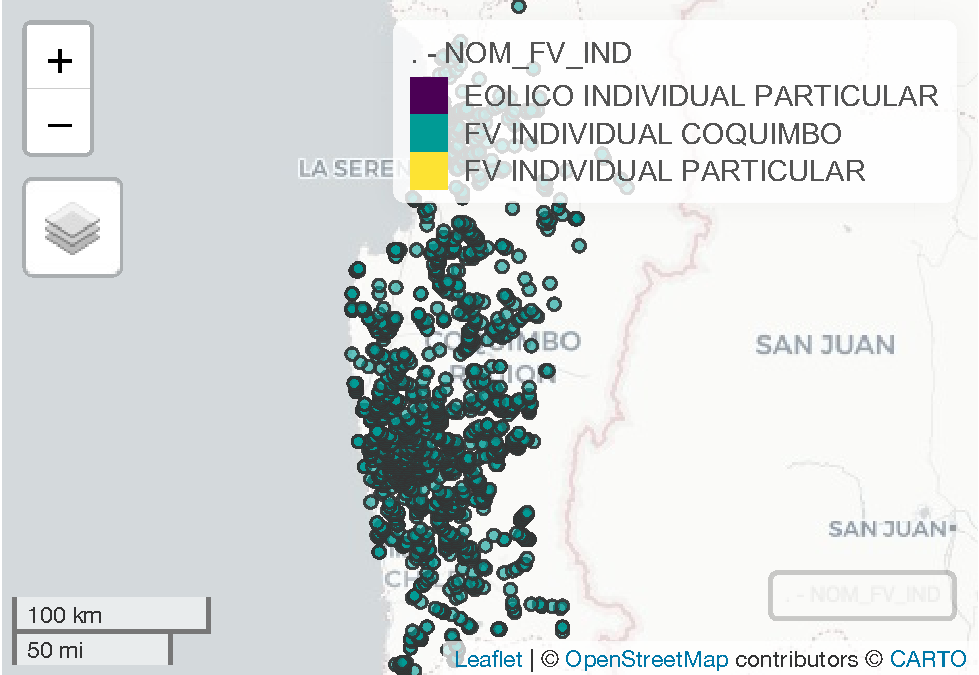
\includegraphics{bookdown_BID_PE_files/figure-latex/unnamed-chunk-26-1.pdf}

\hypertarget{referencias}{%
\chapter{Referencias}\label{referencias}}

\hypertarget{refs}{}
\begin{CSLReferences}{0}{0}
\end{CSLReferences}

  \bibliography{book.bib,packages.bib}

\end{document}
